\documentclass[11pt,norsk]{article}

\usepackage[utf8]{inputenc}
\usepackage[T1]{fontenc,url}
\usepackage[norsk]{babel}
\usepackage{parskip}
\usepackage{lmodern}
\usepackage{microtype}
\usepackage{verbatim}
\usepackage{amsmath, amssymb}
\usepackage{mathtools}
\usepackage{tikz}
\usepackage{physics}
\usepackage{algorithm}
\usepackage{algpseudocode}
\usepackage{listings}
\usepackage{enumerate}
\usepackage{graphicx}
\usepackage{float}
\usepackage{epigraph}
\usepackage{hyperref}
\usepackage[toc,page]{appendix}
\usepackage{varioref}
\usepackage{enumitem}
\usepackage{siunitx}
\usepackage[margin=3cm]{geometry}


\begin{document}

\renewcommand{\exp}{\mathrm{e}^}

\title{FYS2130 - Oblig 13}
\author{
		Jonas Gahr Sturtzel Lunde - \texttt{(jonassl)}
		}
\maketitle
\pagebreak


\section*{Oppgave 1}
Fouriertransformasjon tar ikke hensyn til tid, og brukes der man kan anta at bølgen er periodisk. Wavelettransformasjon foregår over en serie lukkede tidsintervall, og gir derfor også informasjon om hvordan frekvenser endres over tid i et signal.


\section*{Oppgave 2}
Dersom signalets frekvens endrer seg nevneverdig over tid vil fouriertransformasjonen gi lite informasjon om hvordan signalet faktisk ser ut. Dersom signalet også er veldig lokalisert over et kort intervall (bølgepakke) vil fouriertransformasjonen også gi dårlige resultater.


\section*{Oppgave 3}
Wavelettransformasjon er mer avansert å implementere, og krever betydelig mer ressurser å beregne. Utover dette ligger i utgangspunktet all informasjon fra Fourieranalyse også i en Waveletanalyse, men dersom man ser på et periodisk signal er det ingen grunn til å skulle bruke waveletanalyse.


\section*{Oppgave 5}
I randsonene vil bare en andel av waveleten overlappe med signalet vi ser på, og resten vil befinne seg utenfor hele signalområdet. Randområdene vil derfor fremstå med en lavere intensitet enn resten av signalområdet. Når hele waveleten er innenfor signalområdet er denne feilen borte, men frodi waveleten er gaussisk vil det i teorien alltid være deler av den utenfor signalområdet. Vi må altså velge oss et punkt der waveleten er "godt nok" innenfor. Boken har valgt å si at feilen er ubetydelig når bare områdenet av waveleten med amplitude lavere enn $1/e$ av dens maksinale amplitude er utenfor signalområdet.


\section*{Oppgave 8}
\subsection*{a)}
I figur \ref{fig:sinus_wave1} ser vi $f(x)$ i tidsdomenet. Ettersom bølgen har en ekstremt stor frekvens er det vanskelig å tyde figuren. Figur \ref{fig:sinus_wave2} viser et lite utsnitt av bølgen, som gir et bedre inntrykk av hvordan den utvikler seg over tid. Vi kan også se at den er ganske hakkete, grunnet den begrensede oppløsningen av tidspunkter vi bruker.
\begin{figure}[H]
\centering
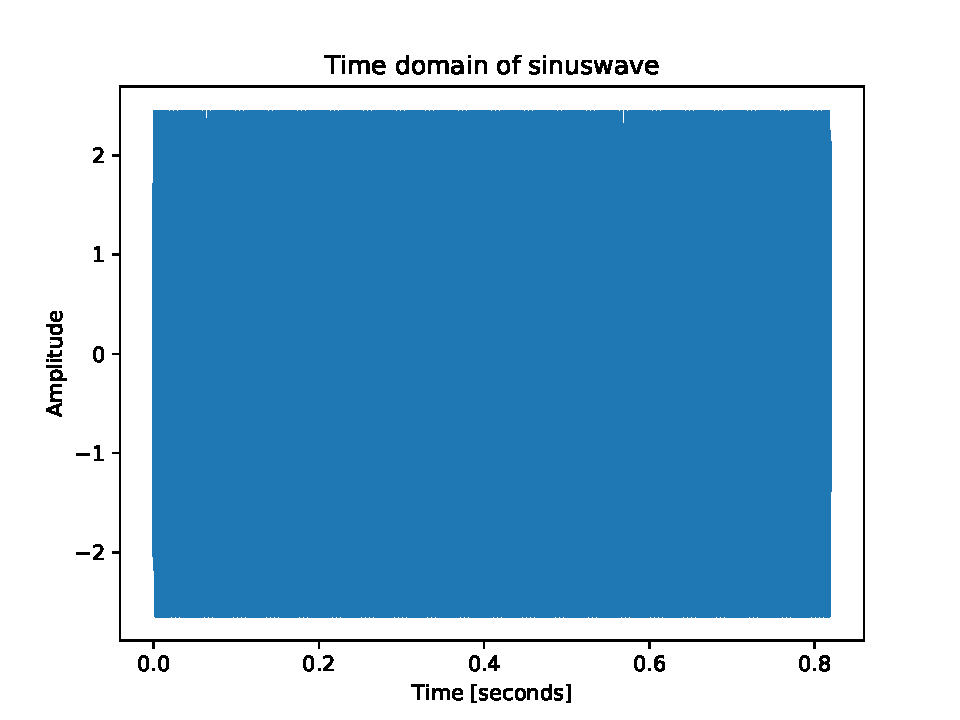
\includegraphics[width=0.8\textwidth]{fig/sinus_wave1.pdf}
\caption{Hele bølgen til f(x) over tid}
\label{fig:sinus_wave1}
\end{figure}

\begin{figure}[H]
\centering
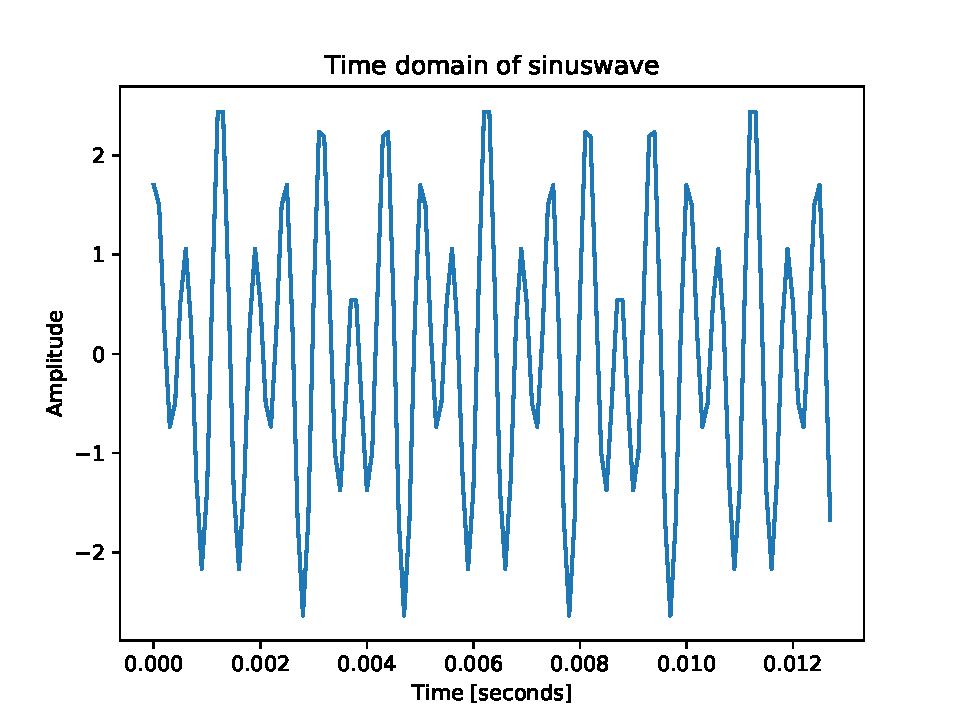
\includegraphics[width=0.8\textwidth]{fig/sinus_wave2.pdf}
\caption{Utsnitt av de første 0.013 sekundene til f(x)}
\label{fig:sinus_wave2}
\end{figure}




\subsection*{b)}
Figur \ref{fig:FT_sinus_wave} ser vi frekvensspekteret til $f(x)$. Vi ser fortsatt topper på våre valgte frekvenser, 1000 og 1600 Hertz. Vi ser også at amplituden er størst på det harmoniske leddet vi har størst koeffisient på.
\begin{figure}[H]
\centering
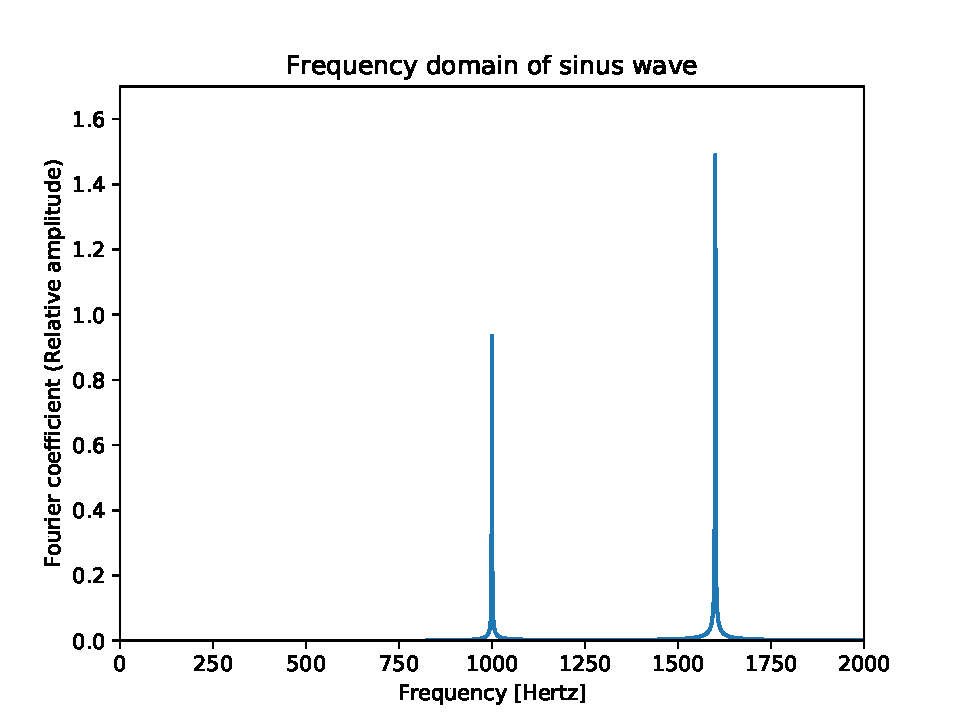
\includegraphics[width=0.8\textwidth]{fig/FT_sinus_wave.pdf}
\caption{Fouriertransformerte av f(x)}
\label{fig:FT_sinus_wave}
\end{figure}



\subsection*{c)}
I figur \ref{fig:wl_sinus_wave1} og \ref{fig:wl_sinus_wave2} ser vi wavelet plottene av $f(x)$ for $k=24$ og $k=200$. Som vi forventet ser vi frekvenser som faller på frekvensene vi valgte. De er også konstante over tid. Vi ser også at at en større K-verdi gir en bedre presisjon i frekvens. Vi merker ikke den dårligere oppløsnignen i tid, fordi frekvensen er konstant over tid.
\begin{figure}[H]
\centering
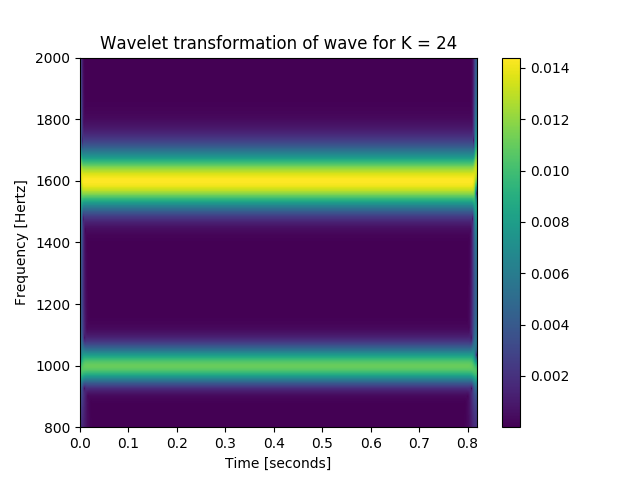
\includegraphics[width=0.8\textwidth]{fig/wavelet_sinus_k=24.png}
\caption{Wavelet transformerte av f(x) med k = 24.}
\label{fig:wl_sinus_wave1}
\end{figure}

\begin{figure}[H]
\centering
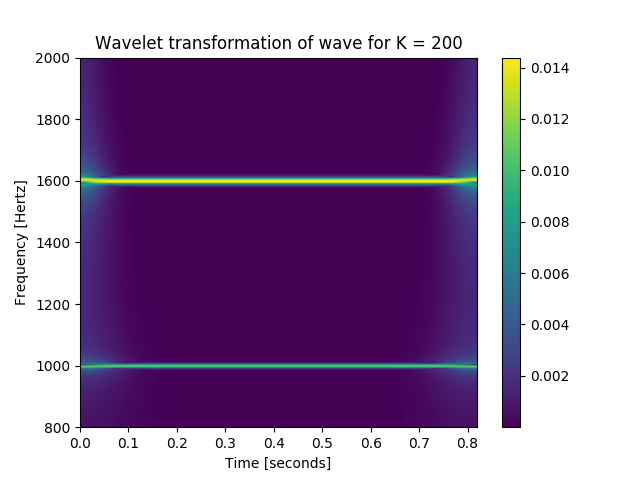
\includegraphics[width=0.8\textwidth]{fig/wavelet_sinus_k=200.png}
\caption{Wavelet transformerte av f(x) med k = 200.}
\label{fig:wl_sinus_wave2}
\end{figure}


\subsection*{d)}
I figur \ref{fig:gaussian_wave} ser vi de to gaussiske bølgene. De består av mange små harmoniske svingninger, omhyllet av en gaussisk kurve.
\begin{figure}[H]
\centering
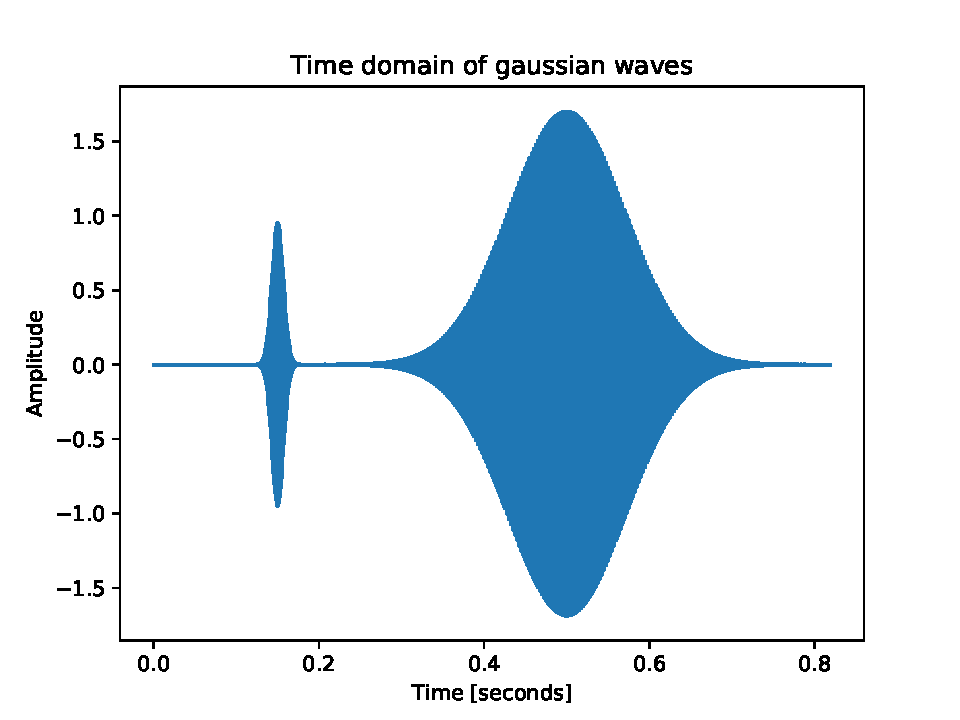
\includegraphics[width=0.8\textwidth]{fig/gaussian_wave.pdf}
\caption{Ny $f(x)$ plottet over tid.}
\label{fig:gaussian_wave}
\end{figure}

Figur \ref{fig:FT_gaussian_wave} viser frekvensspekteret til den nye gaussiske $f(x)$. Vi ser at frekvensene faller rundt de samme områdene som før, men at amplituden er betydelig mindre, og spesielt 1000 Hertz blir mindre veldefinert, sannsynligvis fordi den er veldig lokalisert i tid. Vi ser nå et scenario som fourieranalyse ikke takler så godt som wavelet.
\begin{figure}[H]
\centering
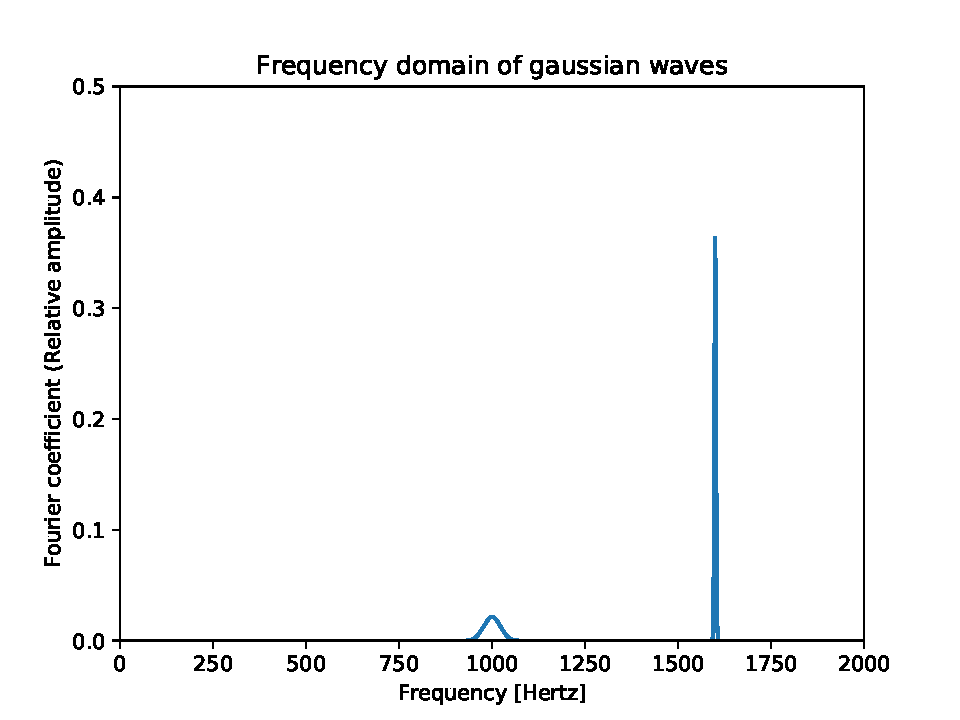
\includegraphics[width=0.8\textwidth]{fig/FT_gaussian_wave.pdf}
\caption{Fouriertransformasjon av ny $f(x)$}
\label{fig:FT_gaussian_wave}
\end{figure}

Figur \ref{fig:wavelet_gaussian_wave1} og \ref{fig:wavelet_gaussian_wave2} viser den wavelettransformerte av de nye gaussiske bølgene for $K = 24$ og $K = 100$. Vi ser at frekvensene fortsatt faller på samme sted, men at de nå er lokalisert på et bestemt punkt i tid. Vi ser også at en høyere K-verdi gir bedre presisjon i frekvens, men nå merker vi at det går på bekostning av presisjonen i tid.
\begin{figure}[H]
\centering
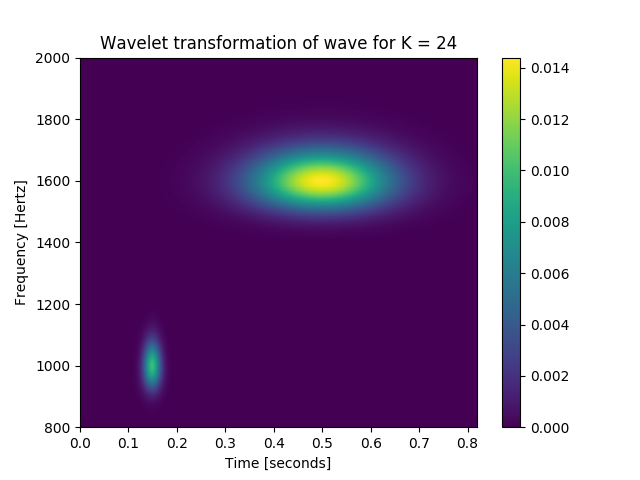
\includegraphics[width=0.8\textwidth]{fig/wavelet_gaussian_k=24.png}
\caption{Wavelettransformerte av gaussbølgene ved $K = 24$.}
\label{fig:wavelet_gaussian_wave1}
\end{figure}

\begin{figure}[H]
\centering
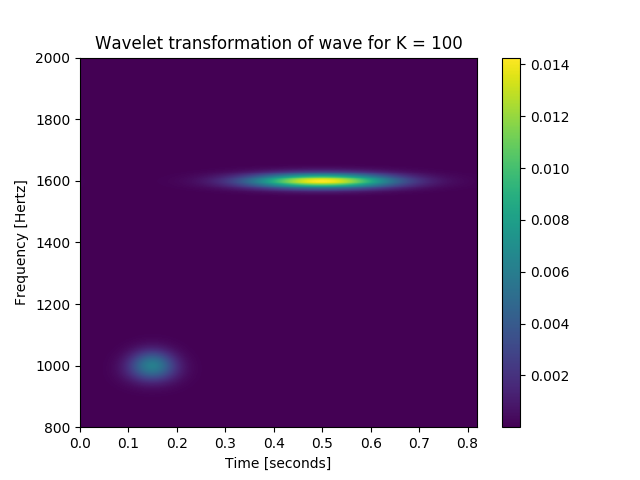
\includegraphics[width=0.8\textwidth]{fig/wavelet_gaussian_k=100.png}
\caption{Wavelettransformerte av gaussbølgene ved $K = 100$.}
\label{fig:wavelet_gaussian_wave2}
\end{figure}

\end{document}
